\section{\texttt{hysteretic}}\label{sec:example_hysteretic}

This example replicates the problem in ``Section 4.3 A Hysteretic Model Class
'' of~\cite{CheungPrudencio2012}, and which is also discussed in \cite{Cheung_2009A}.
In this example we consider the nonlinear seismic response of a four-story building. 
This response is modeled with
an inelastic shear building model with some linear viscous damping and hysteretic bilinear interstory restoring forces~\cite{Cheung_2009A}. More
specifically, let $t\geq0 $ denote time, let $a_g(t)$ be a given total acceleration at the base (Fig. 13), and for the i-th floor [degree of freedom (dof)], $1 \leq i \leq N_o \equiv 4$, let us denote:
\begin{equation}
\begin{split}
m_i &= \text{lumped mass},\\
q_i(t) &= \text{horizontal displacement},\\
F_i(t) &= \text{hysteretic restoring force}
\end{split}
\end{equation}

The hysteretic restoring force is illustrated in Figure \ref{fig:hyst_rest_force} and the horizontal base (ground) acceleration (input data) used in~\cite{CheungPrudencio2012} is illustrated in \ref{hig:hist_base_acceleration}. 
\begin{figure}[h!]
\centerline{
\input{rawfigs/hyst_restoring_force.latex}\\
}
\caption{Illustration of the hysteretic restoring force [see Eq. \eqref{eq:hyst:motion}] used in our hysteretic test problem. The terms $r_i$, $k_i$, and $u_i$ denote model parameters.}
\label{fig:hyst_rest_force}
\end{figure}
%
\begin{figure}[hptb]
\centering
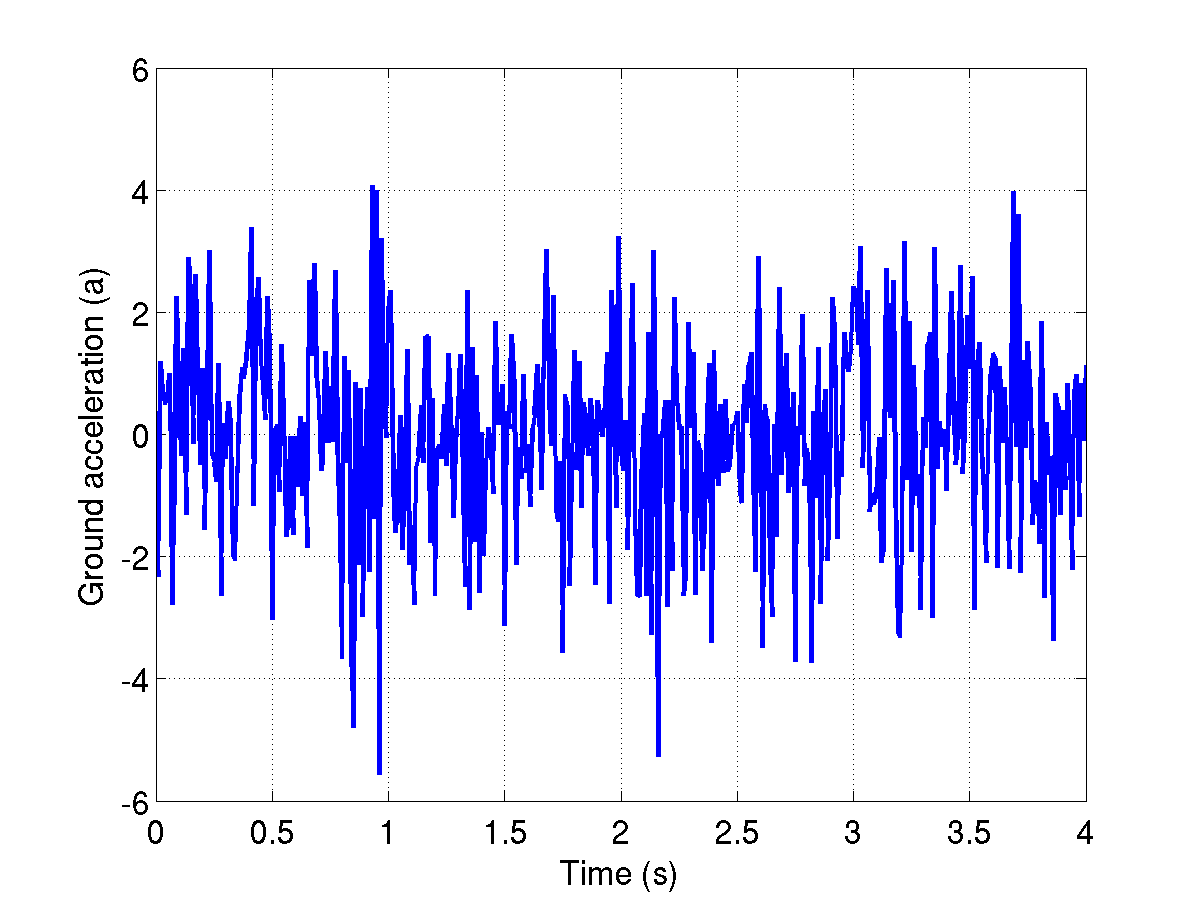
\includegraphics[scale=0.6]{figs/hysteretic_eg_cpp_1.png}
\vspace{-8pt}
\caption{Horizontal base acceleration (input data) used in the hysteretic test problem~\cite{CheungPrudencio2012}.}
\label{hig:hist_base_acceleration}
\end{figure}

We also define the mass matrix $\bv{M}$ and the stiffness matrix $\bv{K}$:
\begin{equation*}
\bv{M}= 
\begin{bmatrix}
  m_1 & 0   & 0   & 0 \\
  0   & m_2 & 0   & 0 \\
  0   & 0   & m_3 & 0 \\
  0   & 0   & 0   & m_4 \\
\end{bmatrix}
%
\quad \text{and} \quad
%
\bv{K}= 
\begin{bmatrix}
  k_1 + k_2 & -k_2    & 0       & 0 \\
  -k_2      & k_2+k_3 & -k_3    & 0 \\
  0         & -k_3    & k_3+k_4 & -k4 \\
  0         &   0     & -k_4    & k_4 \\ 
\end{bmatrix}
\end{equation*}
and the Rayleigh damping matrix
\begin{equation*}
\bv{C} = \rho \bv{M} + \gamma \bv{K} 
\end{equation*}
for given positive scalar parameters $\rho$ and $\gamma$. The response $\bv{q}(t) \equiv [q_1(t),q_2(t),q_3(t),q_4(t)]$ is modeled as satisfying the equation of motion:
\begin{equation}\label{eq:hyst:motion}
\bv{M} \ddot{\bv{q}}(t) + \bv{C} \dot{\bv{q}}(t) + \bv{F}(t) = -\bv{M}\cdot 
\begin{bmatrix} 
1 \\ 
\vdots \\
1
\end{bmatrix}_{4\times1} \cdot a_g(t),
\end{equation}
where $\bv{F}(t) \equiv [F_1(t), F_2(t), F_3(t), F_4(t)]$. In this model, the hysteretic restoring force $\bv{F}(t)$ depends on the whole
time history $[\bv{q}(t),\dot{\bv{q}}(t)]$ of responses from the initial instant until time~$t$.


The (noisy) measured data $y = (y_1, y_2, y_3, y_4)$ available for model calibration consists of 4 s of accelerometer data at each floor (refer to Fig. \ref{hig:hist_acceleration_4_floors}), with a sample interval $\Delta t = 0.01$ s. The simulated dynamic data was obtained by adding Gaussian white noise to the output simulation of the hysteretic model with the following input values:
\begin{align*}
m_1 & = m_2 = m_3 = m_4 = 2\times 10^4 \,kg,\\
k_1 &=  2.2 \times 10^7 \,Nm^{-1},\\
k_2 &=  2.0 \times 10^7 \,Nm^{-1},\\
k_3 &=  1.7 \times 10^7 \,Nm^{-1},\\
k_4 &=  1.45 \times 10^7 \,Nm^{-1},\\
r_1 & = r_2 = r_3 = r_4 = 0.1,\\
u_1 & = u_2 = 8 \times 10^{-3} \,m, \\
u_3 & = u_4 = 7 \times 10^{-3} \,m, \\
\rho &= 7.959 \times 10^{-1}, \\
\gamma &= 2.5 \times 10^{-3},\\
\sigma^2 &= 0.6^2,
\end{align*}
where for $i=1,2,3,4$, $k_i$ is the initial stiffness, $r_i$ is the post-yield stiffness reduction factor, and $u_i$ is  yield displacement.


\begin{figure}[hptb]
\centering
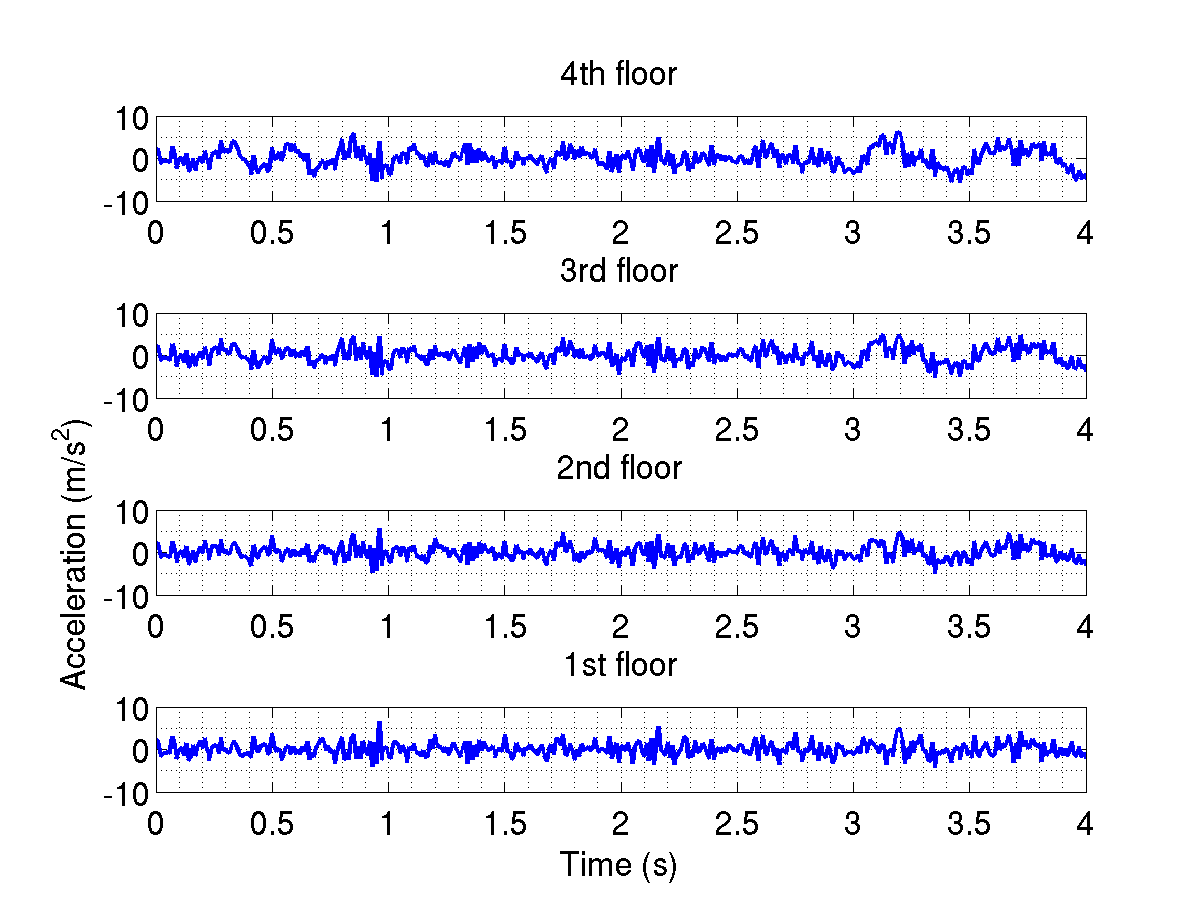
\includegraphics[scale=0.6]{figs/hysteretic_eg_cpp_4.png}
\vspace{-8pt}
\caption{Horizontal acceleration of each of the four floors (measured data aimed for calibration) used in our hysteretic test problem.}
\label{hig:hist_acceleration_4_floors}
\end{figure}

According to Cheung and Prudencio~\cite{CheungPrudencio2012}, these input values were chosen deliberately so that the excitation $a_g$ did not cause some of the upper floors to enter the nonlinear regime; that is, so that our test inverse problem did not become globally identifiable. 

In this section, 400 time-steps are used, as the data is  available  at instants  
$$t_n = (n - 1) \times \Delta t, \quad 1 \leq n \leq N_T \equiv 401, \quad \Delta t = 0.01$$
however, Cheung and Prudencio used only 250 time steps~\cite{CheungPrudencio2012}. 

An additive noise is assumed to be present in the measurements; i.e.,
\begin{equation*}
y_i(n)=q_i(n)+\varepsilon_i(n), \quad 1 \leq i \leq N_o, \quad  1 \leq n \leq N_T \equiv 401, 
\end{equation*}
where $q_i(n; \theta_2 ,...,\theta_{15})$ denotes the output at time $t_n= n\Delta t \, (\Delta t=0.01s)$ at the $i$-th observed degree of freedom predicted by the proposed structural model, and $y_i(n)$ denotes the corresponding
measured output.


They considered a total of 15 unknown parameters $\bv{\theta} = (\theta_1 , . . . , \theta_{15})$ and modeled the variables $\varepsilon_i$ as independently and identically distributed Gaussian variables with mean zero and some unknown prediction-error variance $\sigma^2$. The variance $\sigma^2$ is assumed to be the same for all $N_o = 4$ floors.  The first component $\theta_1$ is equal to the prediction error variance $\sigma^2$ and the other 14 parameters are related to the four triples $(k_i, r_i, u_i),\, 1 \leq i \leq N_o$ (see Fig. \ref{fig:hyst_rest_force}), to $\rho$, and to $\gamma$. The likelihood function is given by:
\begin{equation}\label{eq:hyst:like}
 f(\bv{y}|\bv{\theta}) = \dfrac{1}{(2 \pi \sigma^2)^{N_oN_T/2}}\exp \left( -\dfrac{1}{2\sigma^2} \displaystyle \sum_{i=1}^{N_o} \sum_{n=1}^{N_T} [y_i(t_n) - {q}_i(t_n; \theta_2,\ldots,\theta_{15})]^2 \right).
\end{equation}
An inverse gamma  prior was used for $\theta_1=\sigma^2$, and a 14-dimensional Gaussian prior was used for $\theta_2 , ..., \theta_{15}$ with zero mean and diagonal covariance matrix equal to a scaled identity matrix.


\subsection{Running the Example}\label{sec:hysteretic-run}

To run the executable provided (available after QUESO installation), and generate figures for the chains, KDEs, CDFs, autocorrelation and scatter plots, enter the following commands:
\begin{lstlisting}[label={},caption={}]
$ cd $HOME/LIBRARIES/QUESO-0.51.0/examples/example
$ rm outputData/*
$ ./example_gsl example_1chain.inp    
$ matlab
   $ plot_all.m	                          # inside matlab   
$ ls -l outputData/*.png
hysteretic_autocorr_thetas.png  hysteretic_kde_theta8.png 
hysteretic_cdf_thetas.png       hysteretic_kde_theta9.png
hysteretic_kde_theta1.png       hysteretic_kde_theta10.png
hysteretic_kde_theta2.png       hysteretic_kde_theta11.png
hysteretic_kde_theta3.png       hysteretic_kde_theta12.png
hysteretic_kde_theta4.png       hysteretic_kde_theta13.png
hysteretic_kde_theta5.png       hysteretic_kde_theta14.png
hysteretic_kde_theta6.png       hysteretic_kde_theta15.png
hysteretic_kde_theta7.png       hysteretic_scatter_thetas.png
\end{lstlisting}


As a result, the user should have created several of PNG figures containing kernel density estimate of the 15 parameters, cumulative density distribution, autocorrelation and scatter plots. The name of the figure files have been chosen to be informative, as shown in the Listing above.

Additional figures may be generated if the user allows the procedure \texttt{debug\_hyst(} be called by the compiler in Line 11 of file \texttt{example\_main.C}; in that case, call the function \texttt{cpp\_gen.m} inside Matlab/Octave. 


\subsection{Example Code}\label{sec:hysteretic-code}

The source code for the example is composed of 5 files:
\texttt{example\_main.C} (Listing \ref{code:hysteretic-main-c}), \linebreak
\texttt{example\_likelihood.h} and \texttt{example\_likelihood.C} (Listings \ref{fig-like-example-h} and \ref{fig-like-example-c}),
\texttt{example\_compute.h} and \texttt{example\_compute.C} (Listings \ref{code:hysteretic-compute-h} and \ref{code:hysteretic-compute-c}), and finally \texttt{example\_hyst.h} and \texttt{example\_hyst.C}, which contain the Hysteretic model properly said.


Note that in line 11 of Listings \ref{code:hysteretic-main-c} the `\verb+#if 1+' directive tells the compiler that the application will call \texttt{compute()}, which internally uses QUESO and the Multilevel algorithm. 
On the contrary, the user may calculate the hysteretic force without uncertainty by changing the directive to `\verb+#if 0+', which can assist the analysis of the resulting data.

\lstinputlisting[caption=File \texttt{example\_main.C.}, label={code:hysteretic-main-c}, linerange={33-1000},numbers=left]{../../examples/hysteretic/src/example_main.C}

\lstinputlisting[caption=File \texttt{example\_likelihood.h}., label={fig-like-example-h}, linerange={33-1000}]{../../examples/hysteretic/src/example_likelihood.h}

\lstinputlisting[caption=File \texttt{example\_likelihood.C}., label={fig-like-example-c}, linerange={33-1000}]{../../examples/hysteretic/src/example_likelihood.C}

\lstinputlisting[caption=File \texttt{example\_compute.h.}, label={code:hysteretic-compute-h}, linerange={33-1000}]{../../examples/hysteretic/src/example_compute.h}

\lstinputlisting[caption={File \texttt{example\_compute.C}.}, label={code:hysteretic-compute-c}, linerange={33-1000}]{../../examples/hysteretic/src/example_compute.C}
 


\subsection{Input File}\label{sec:hysteretic-input-file}


The options used for solving this example are displayed in Listing \ref{code:hysteretic-input-file}. 

\lstinputlisting[caption={Options for QUESO library used in application code (Listings \ref{code:hysteretic-main-c}-\ref{code:hysteretic-compute-c}})., 
label={code:hysteretic-input-file},]{../../examples/hysteretic/tests/test_2013_12_11/example.inp}

\subsection{Create your own Makefile}\label{sec:hysteretic-makefile}

Similarly to the other examples presented in this user's manual and also available with QUESO distribution, a user-created makefile is available: `\texttt{Makefile\_hysteretic\_violeta}' which may personalized to each user's computer settings and used to compile the code and create the executable \verb+hysteretic_gsl+. 

Thus to compile, build and execute the code,  commands similar to the following should be entered:
\begin{lstlisting}
$ cd $HOME/LIBRARIES/QUESO-0.51.0/examples/hysteretic/
$ export LD_LIBRARY_PATH=$LD_LIBRARY_PATH:\
  $HOME/LIBRARIES/gsl-1.15/lib/:\
  $HOME/LIBRARIES/boost-1.53.0/lib/:\
  $HOME/LIBRARIES/hdf5-1.8.10/lib:\
  $HOME/LIBRARIES/QUESO-0.51.0/lib 
$ make -f Makefile_hysteretic_violeta 
$ ./hysteretic_gsl example.inp
\end{lstlisting}

Again, the `\verb+export+' instruction above is only necessary if the user has not saved the path for the libraries used during QUESO installation in his/her \verb+.bashrc+ file. 



\subsection{Data Post-Processing and Visualization}\label{sec:hysteretic-results}



According to the specifications of the input file in Listing~\ref{code:hysteretic-input-file}, both a folder named \verb+outputData+ and a the following files should be generated:
\begin{verbatim}
rawChain_ml.m 
display_sub0.txt    
\end{verbatim}

Note that in this hysteretic problem a total of 13 levels are required for the Multilevel method (e.g. see the contents of file \texttt{rawChain\_ml.m}).

The sequence of Matlab commands is identical to the ones presented in Sections
\ref{sec:sip-results}, \ref{sec:sfp-results}, \ref{sec:gravity-results} and \ref{sec:tga-results};
therefore, are omitted here. The reader is invited to explore the Matlab files
\texttt{plot\_all.m} and/or  \texttt{cpp\_gen.m},  for details of how the figures have been generated.



\subsubsection{KDE Plots}

Figure \ref{fig:hysteretic_kde} presents the KDE plots of each parameter $\theta_i,\, i=1,\ldots,15$.
The Multilevel method also provides data about the logarithm of the likelihood function as well as of the target PDF.
Figure \ref{fig:hysteretic_kde_like} presents the KDE plots of both the likelihood function and of its logarithm.



\begin{figure}[hptb]
\centering
\subfloat{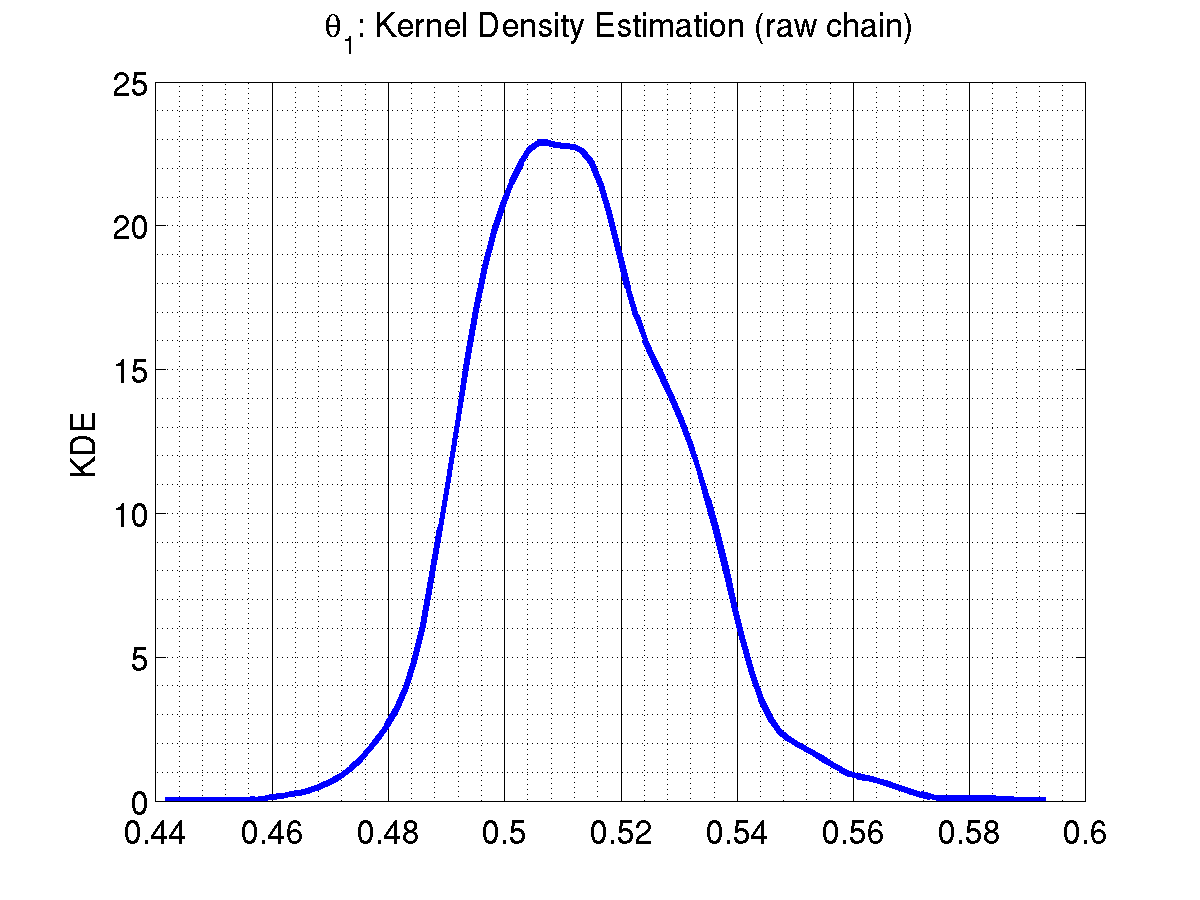
\includegraphics[scale=0.25]{figs/hysteretic_kde_theta1.png}}
\subfloat{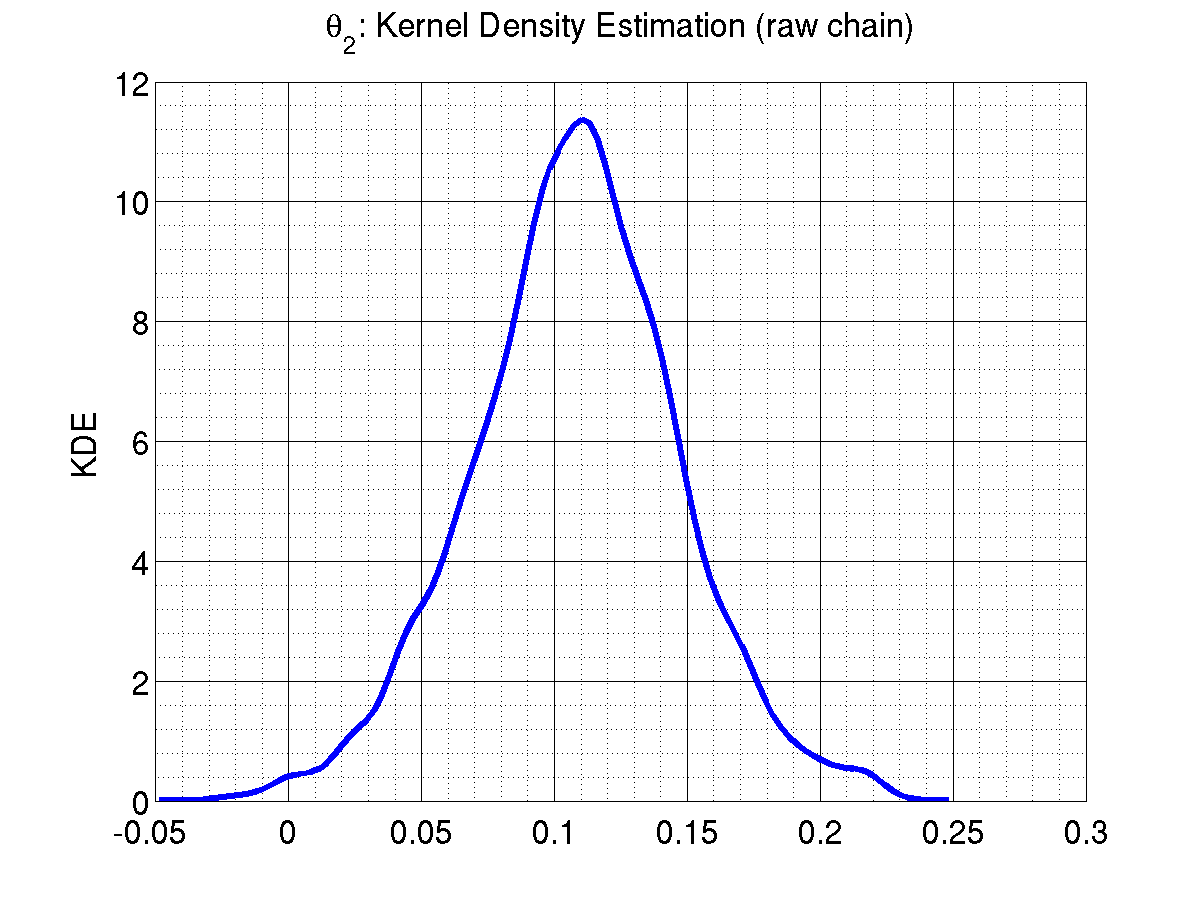
\includegraphics[scale=0.25]{figs/hysteretic_kde_theta2.png}}
\subfloat{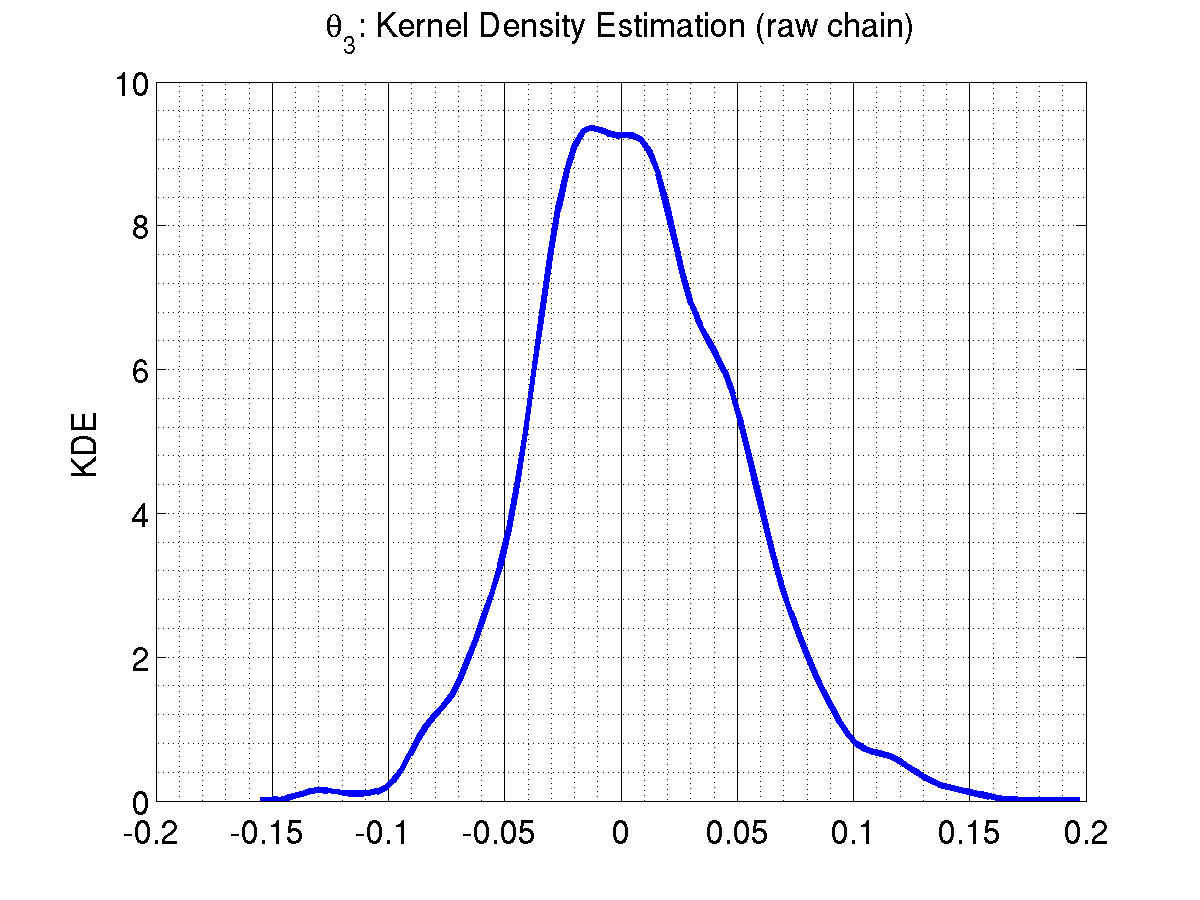
\includegraphics[scale=0.25]{figs/hysteretic_kde_theta3.png}}\\
\subfloat{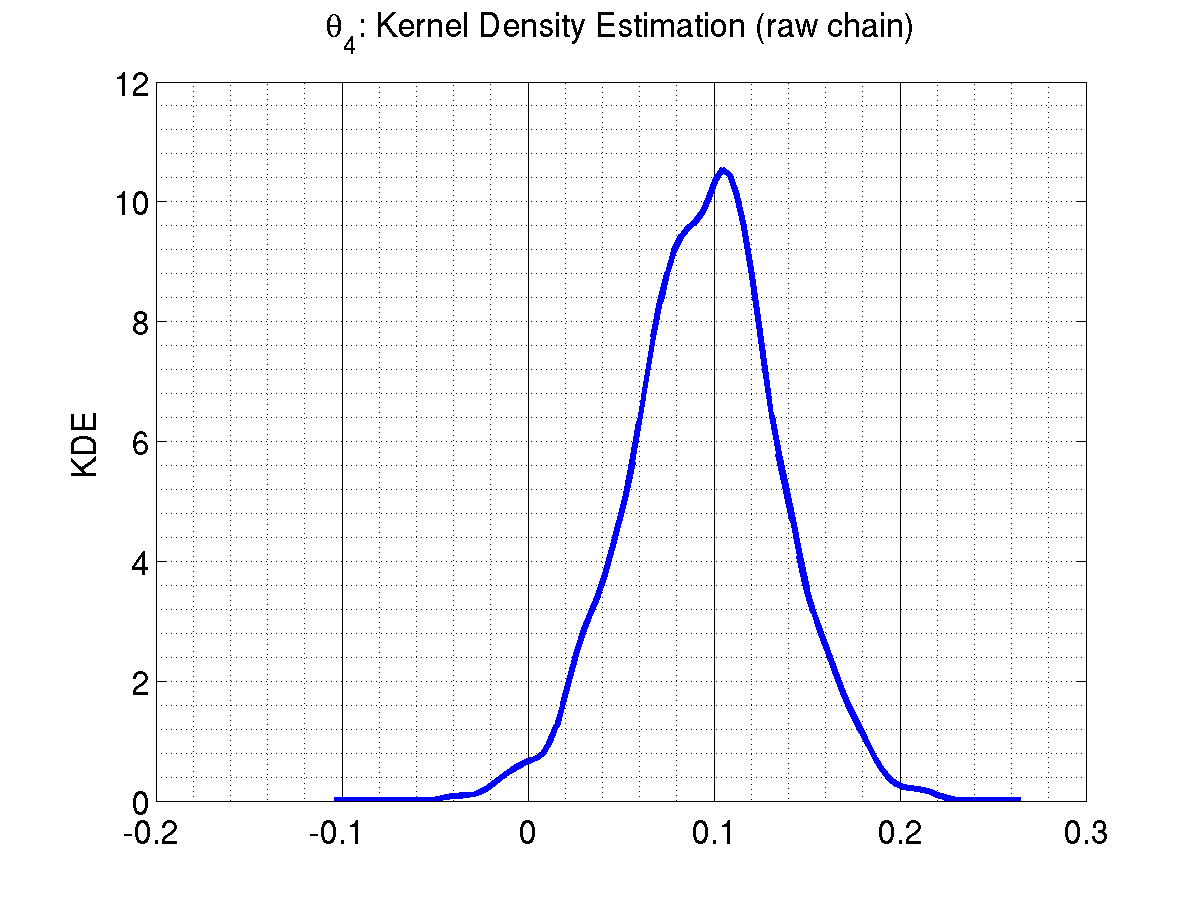
\includegraphics[scale=0.25]{figs/hysteretic_kde_theta4.png}}
\subfloat{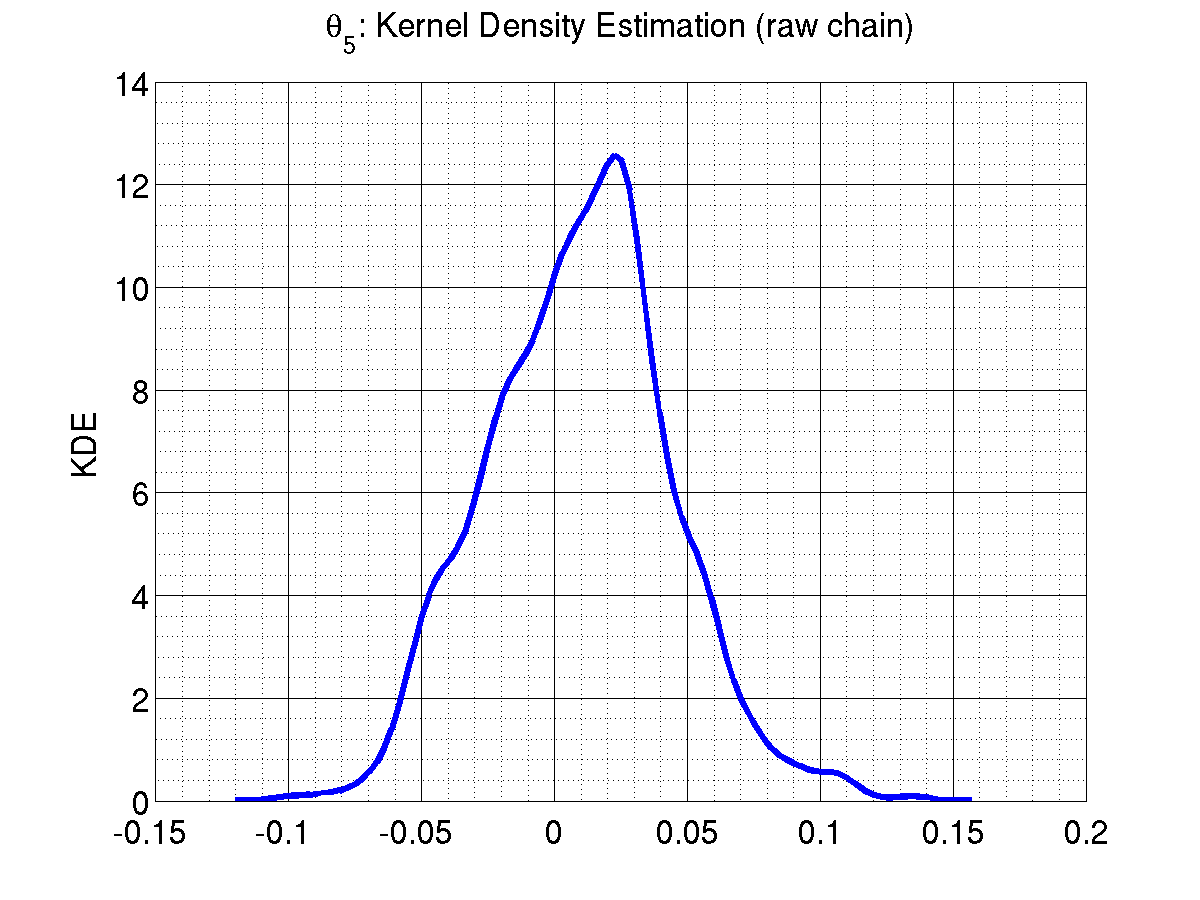
\includegraphics[scale=0.25]{figs/hysteretic_kde_theta5.png}}
\subfloat{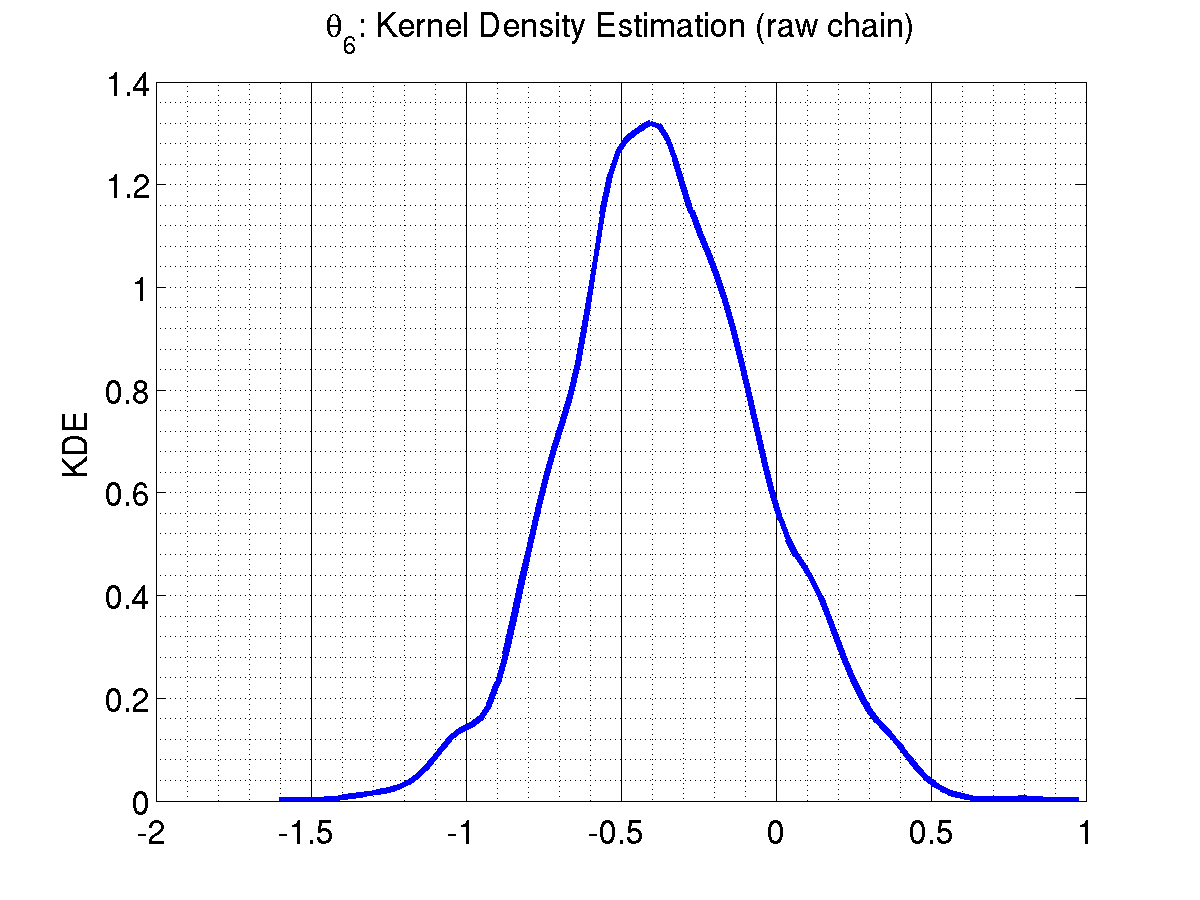
\includegraphics[scale=0.25]{figs/hysteretic_kde_theta6.png}}\\
\subfloat{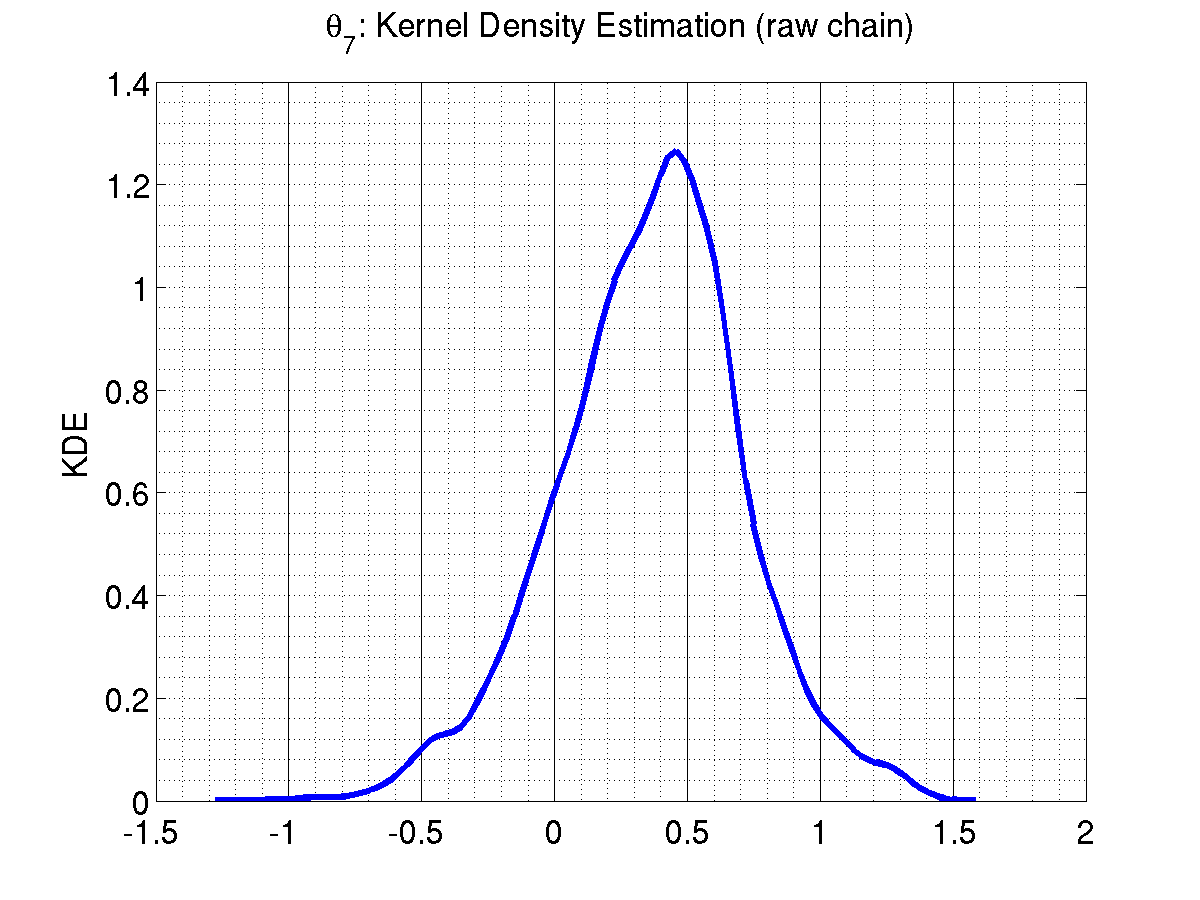
\includegraphics[scale=0.25]{figs/hysteretic_kde_theta7.png}}
\subfloat{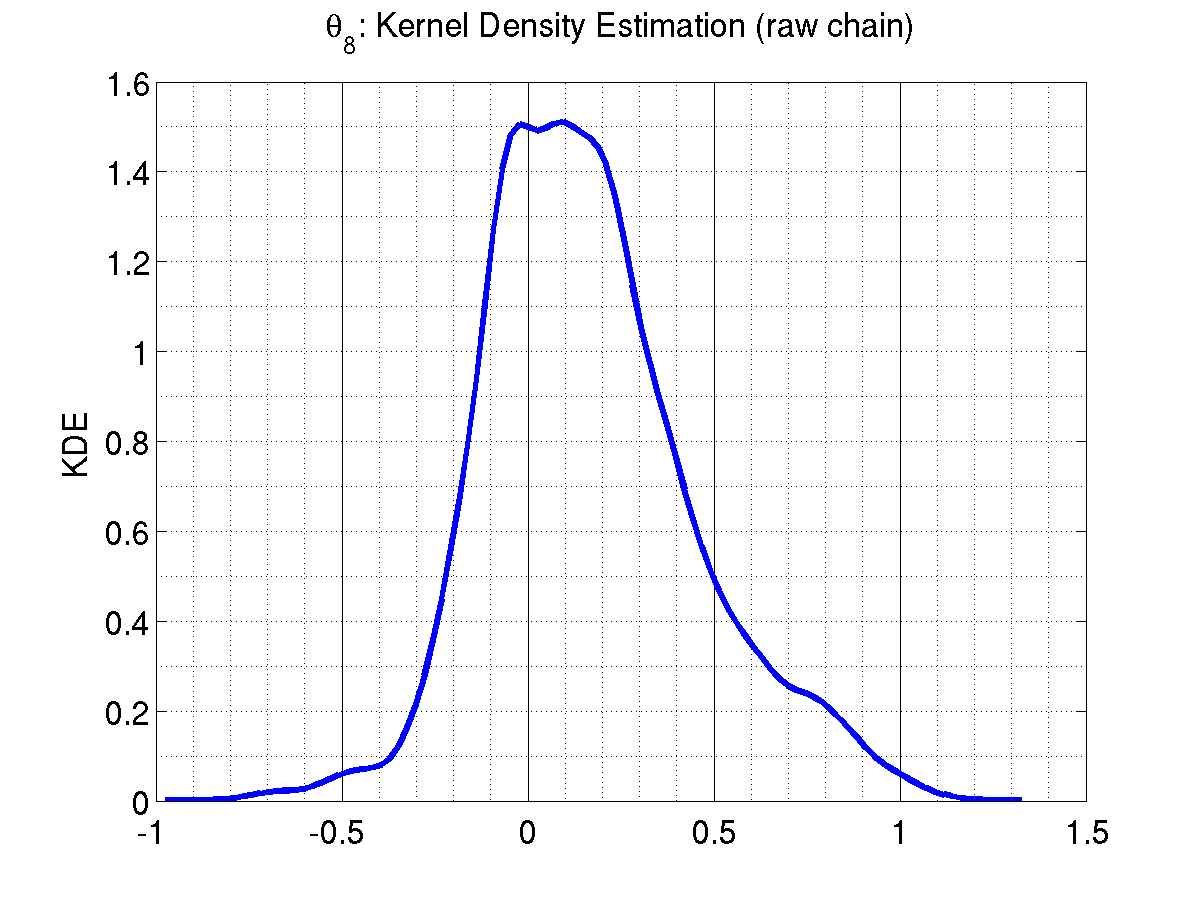
\includegraphics[scale=0.25]{figs/hysteretic_kde_theta8.png}}
\subfloat{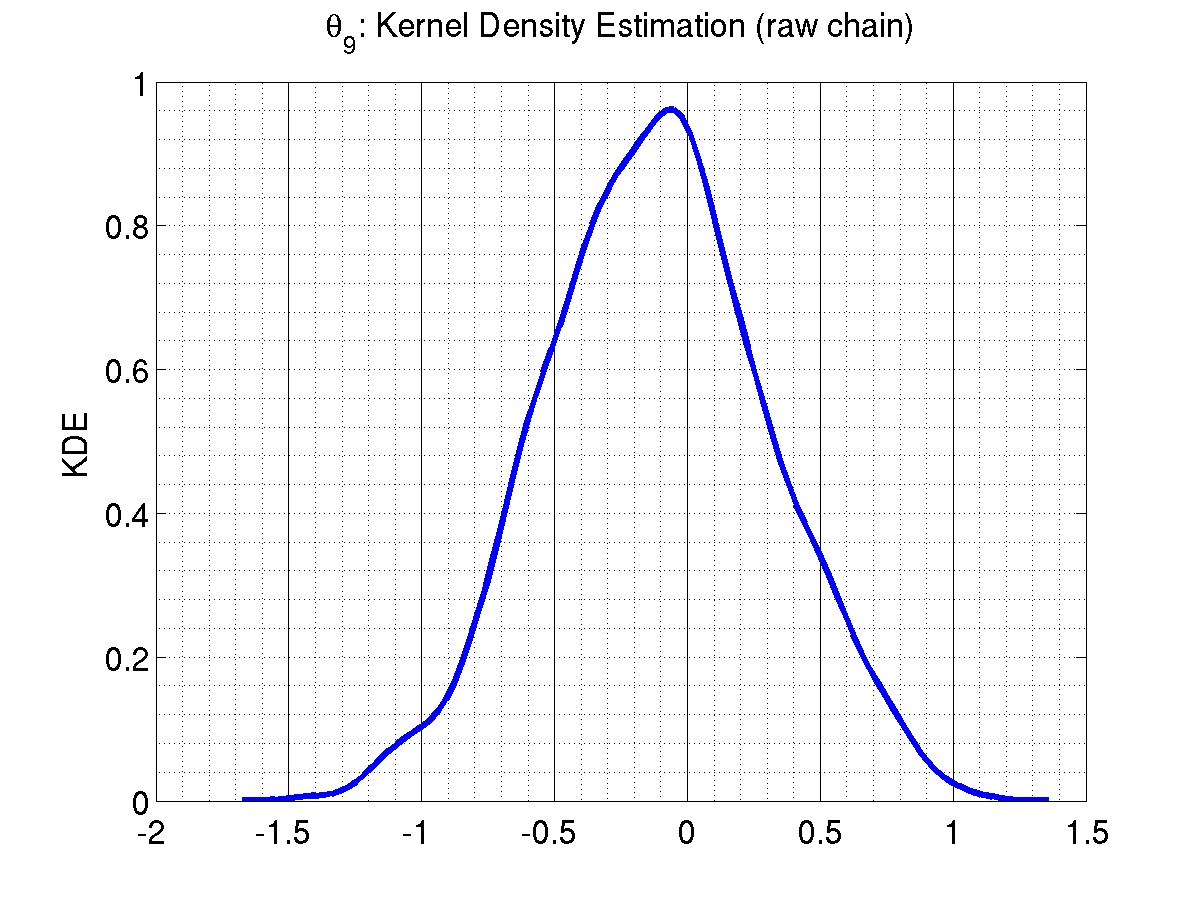
\includegraphics[scale=0.25]{figs/hysteretic_kde_theta9.png}}\\
\subfloat{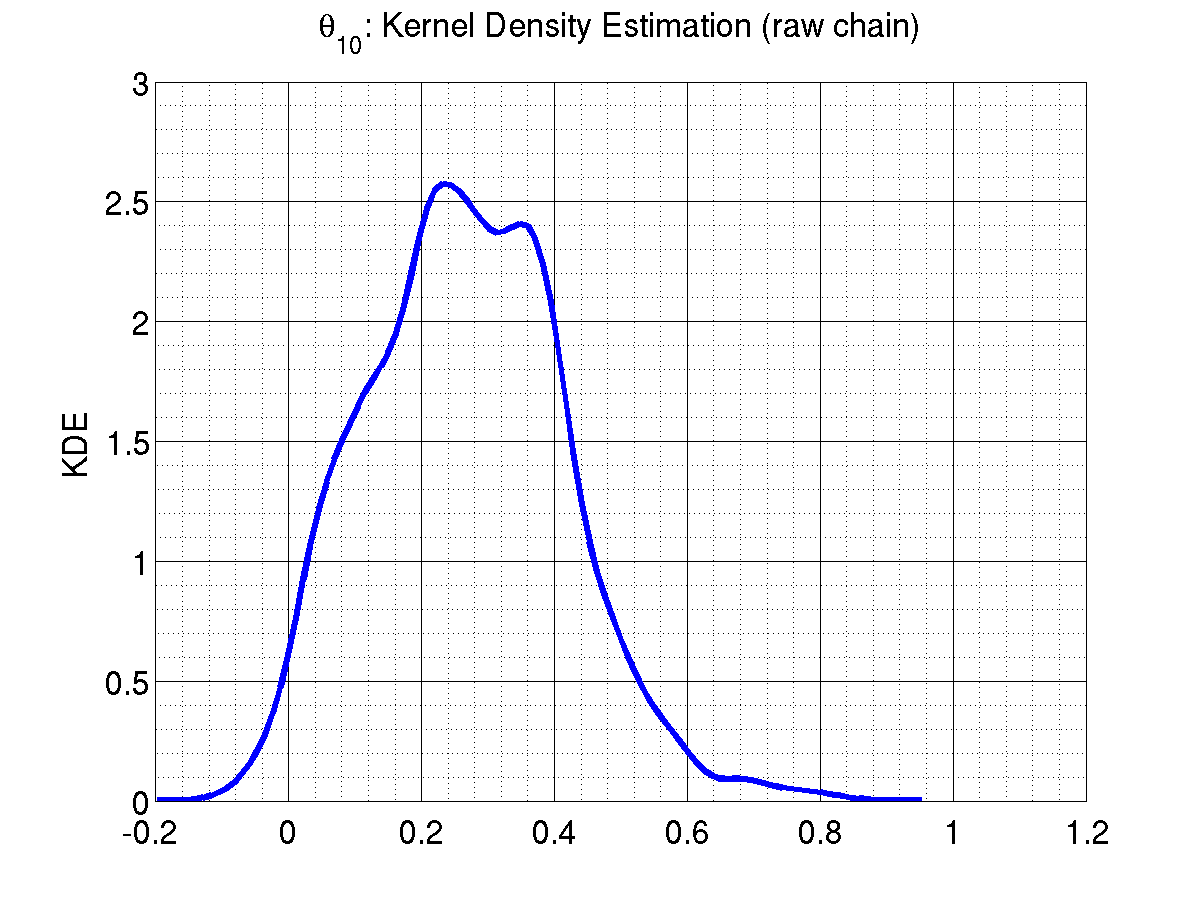
\includegraphics[scale=0.25]{figs/hysteretic_kde_theta10.png}}
\subfloat{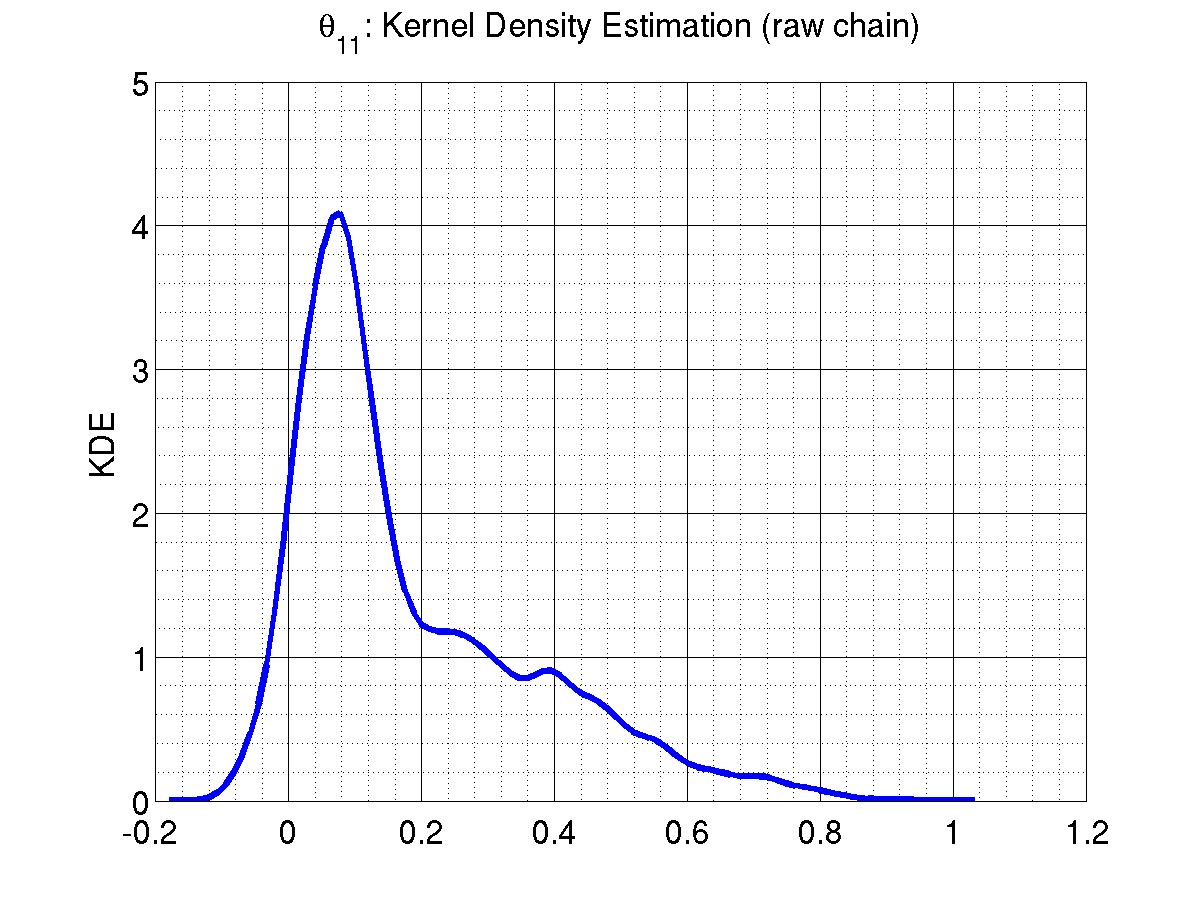
\includegraphics[scale=0.25]{figs/hysteretic_kde_theta11.png}}
\subfloat{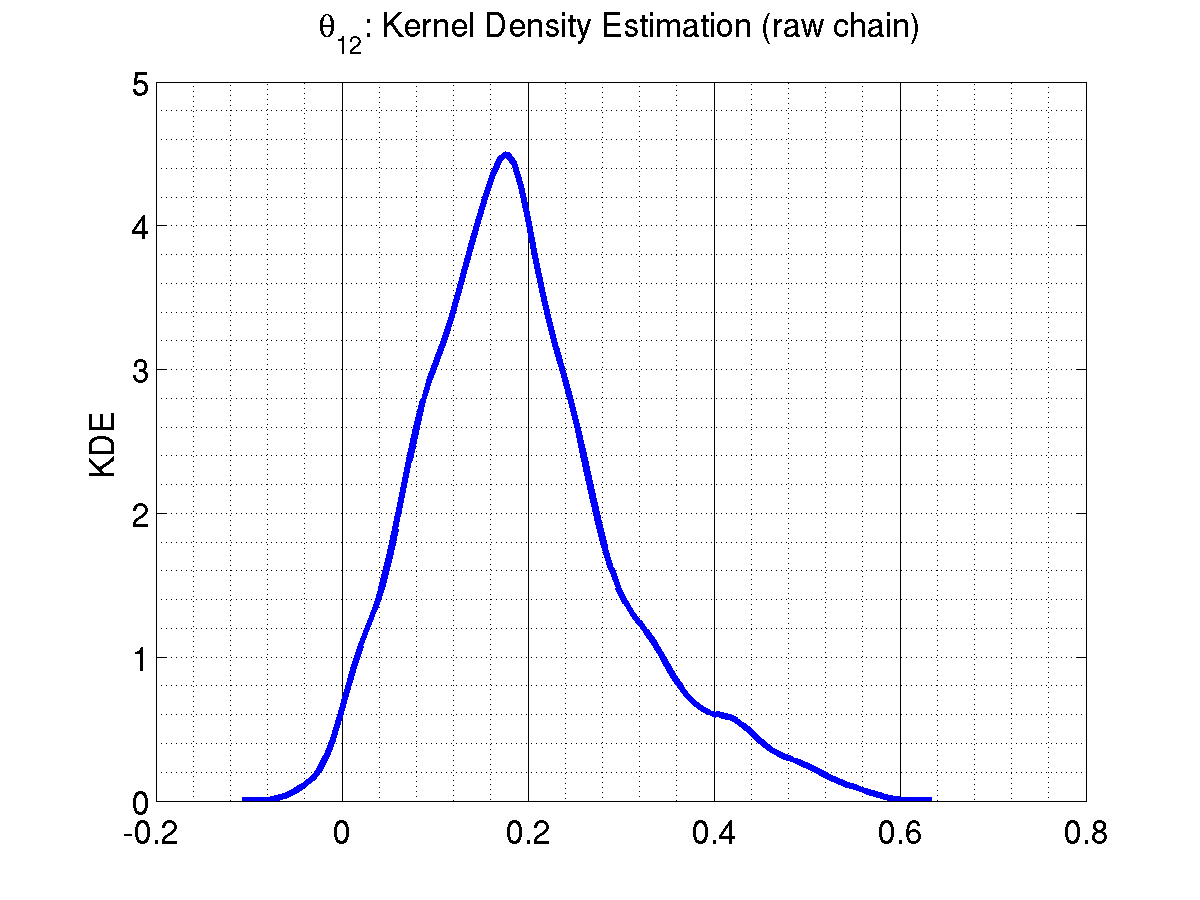
\includegraphics[scale=0.25]{figs/hysteretic_kde_theta12.png}}\\
\subfloat{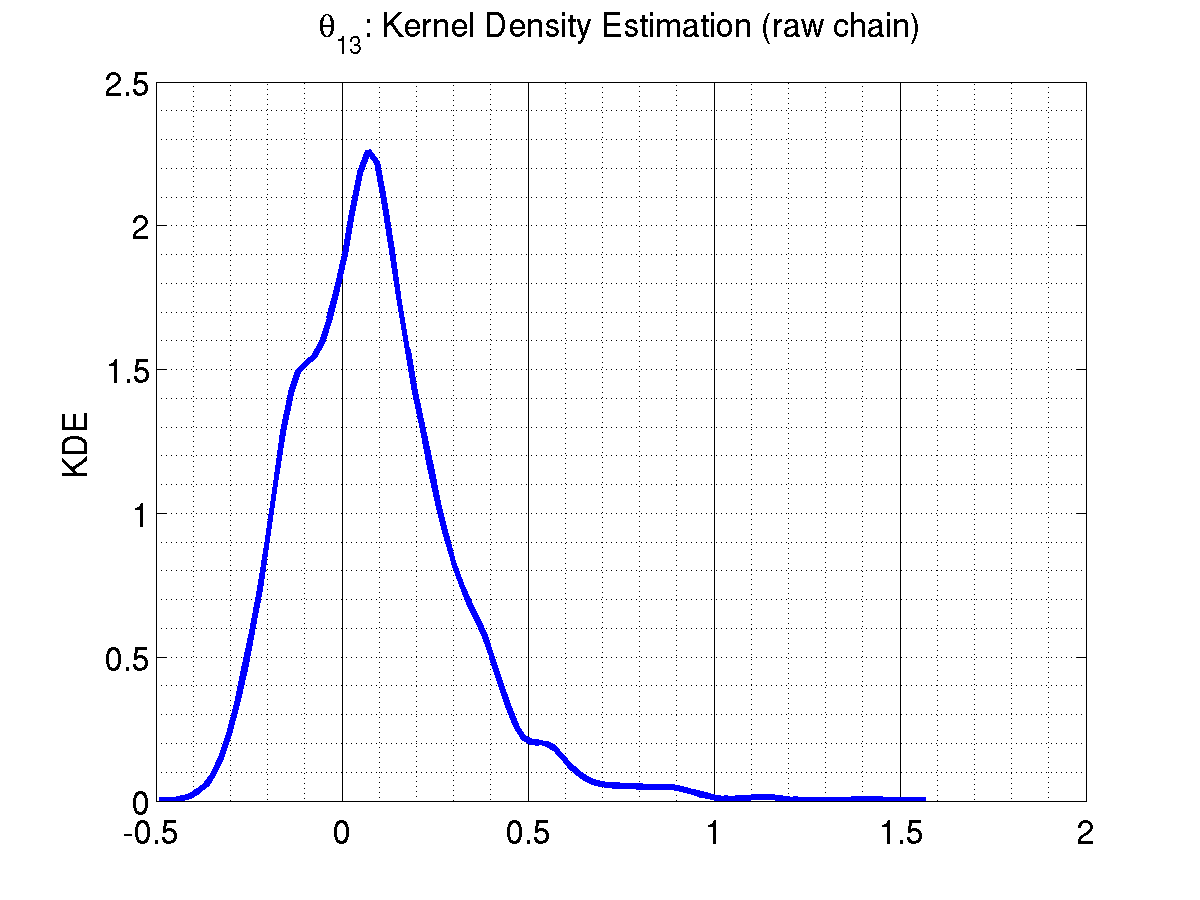
\includegraphics[scale=0.25]{figs/hysteretic_kde_theta13.png}}
\subfloat{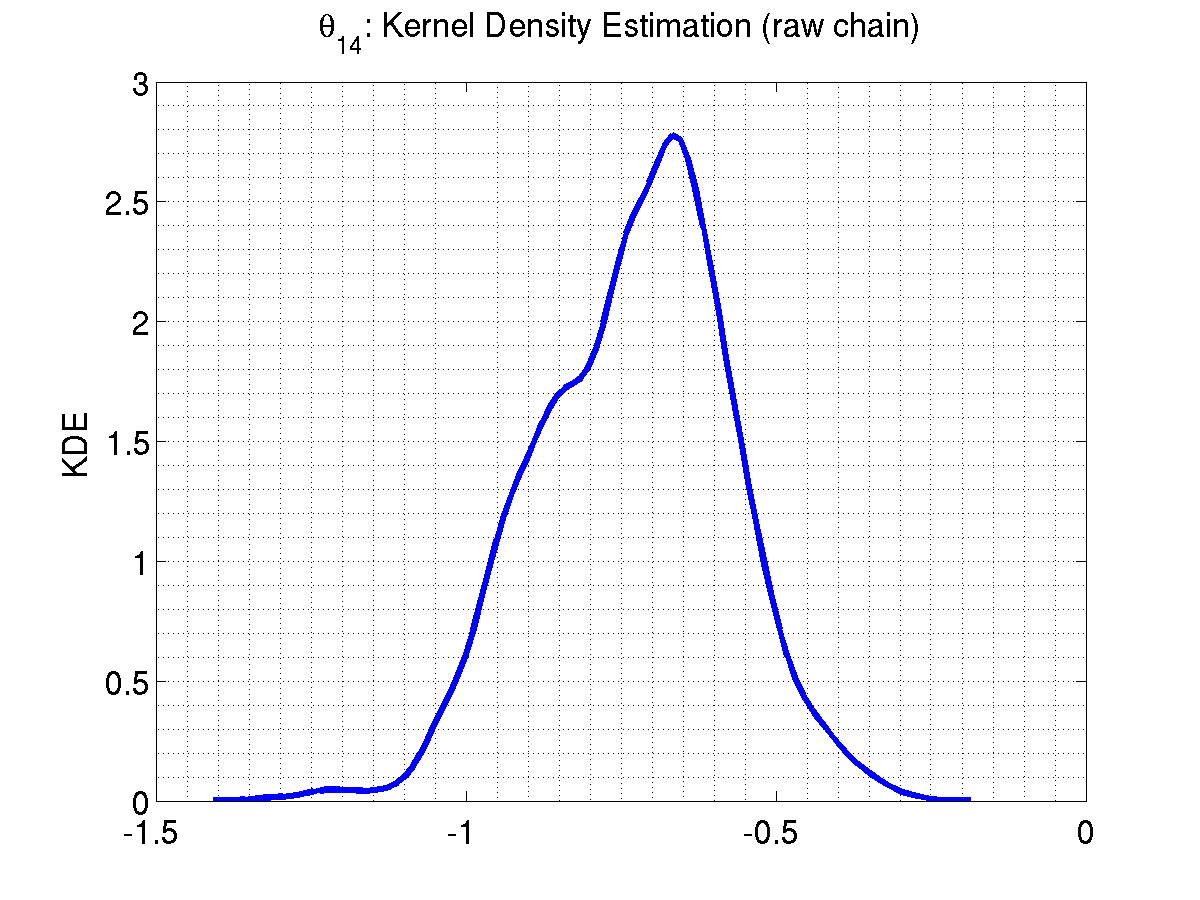
\includegraphics[scale=0.25]{figs/hysteretic_kde_theta14.png}}
\subfloat{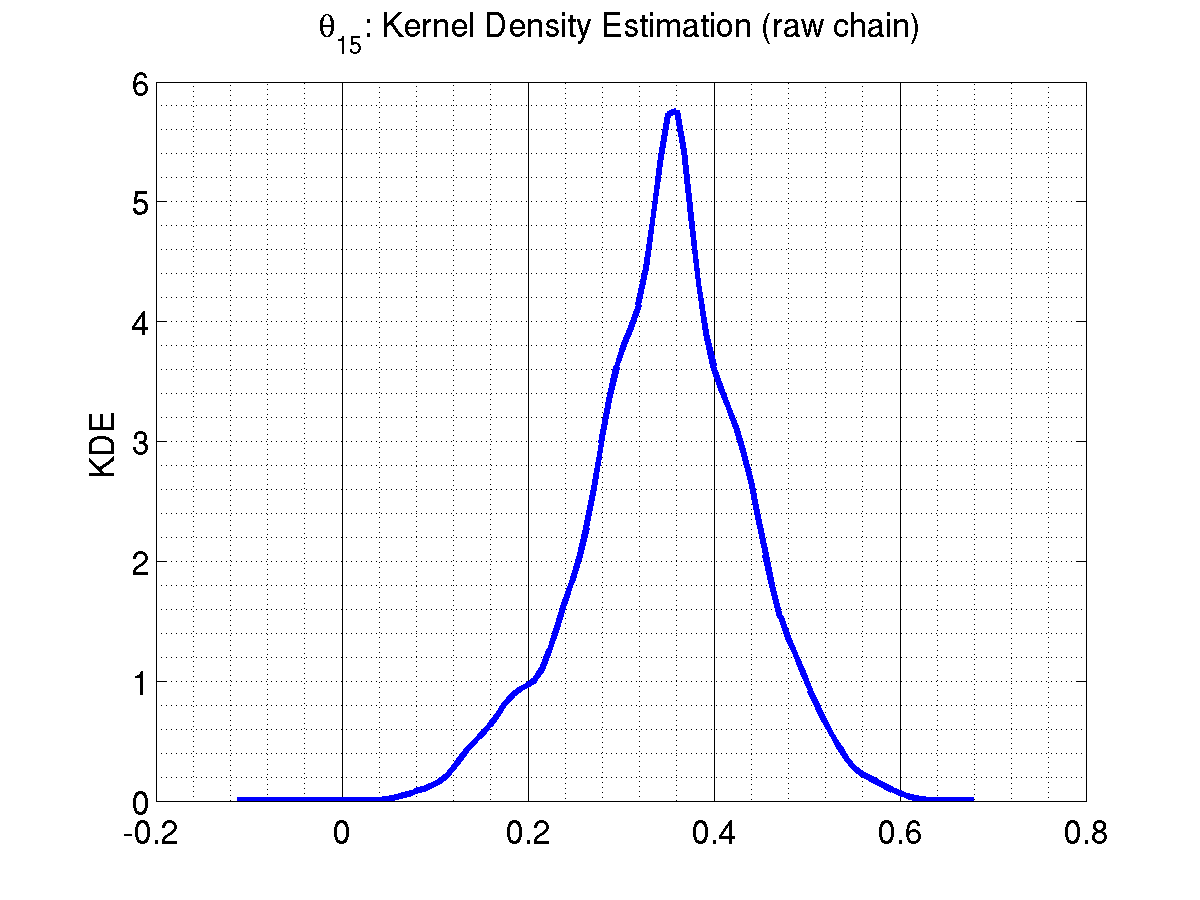
\includegraphics[scale=0.25]{figs/hysteretic_kde_theta15.png}}
\caption{KDE plots of parameter $\bv{\theta}$ at the last level.}
\label{fig:hysteretic_kde}
\end{figure}


\begin{figure}[hptb]
\centering
\subfloat[$\log( f(\bv{y}|\bv{\theta}) )$]{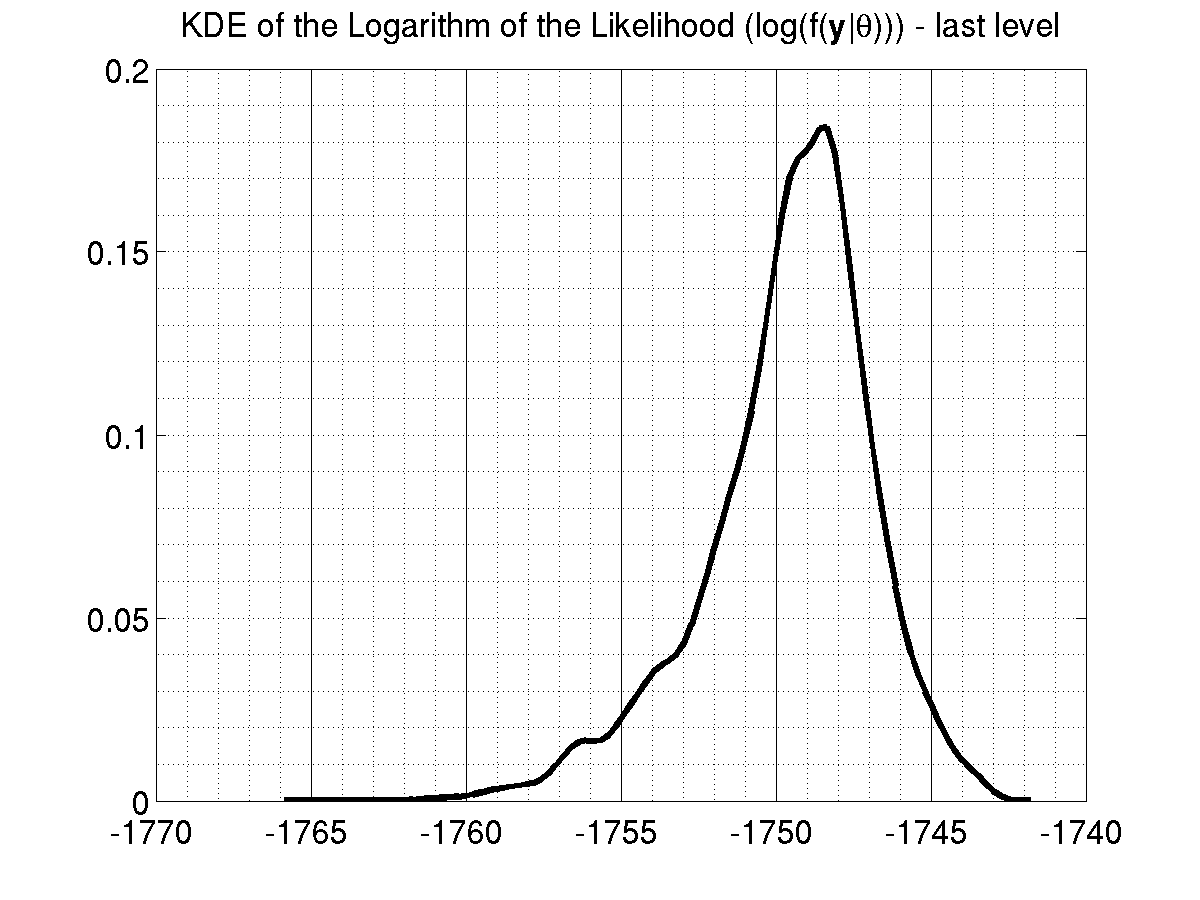
\includegraphics[scale=0.4]{figs/hysteretic_kde_log_likelihood.png}}
\subfloat[$f(\bv{y}|\bv{\theta})$]{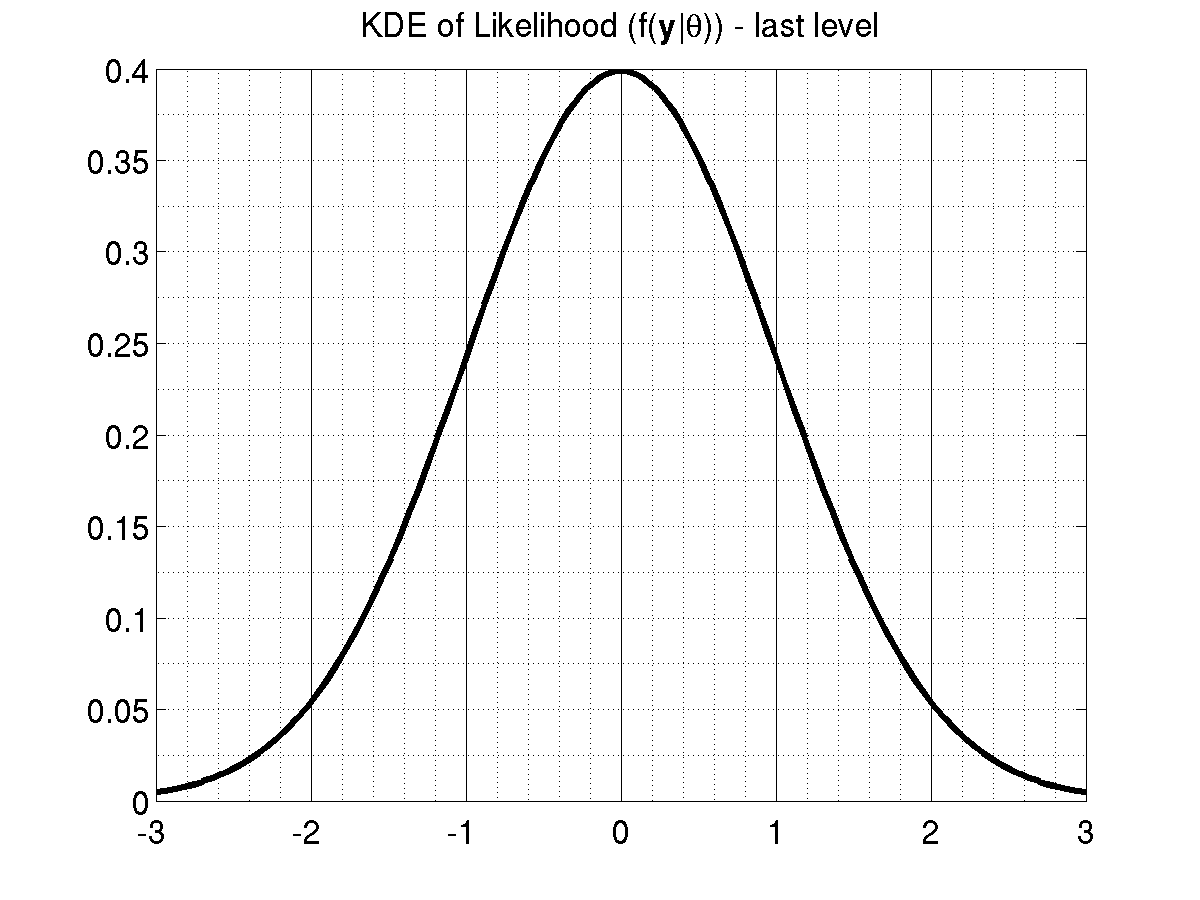
\includegraphics[scale=0.4]{figs/hysteretic_kde_likelihood.png}}
\vspace{-8pt}
\caption{KDE plots of the likelihood function, given by Eq. \eqref{eq:hyst:like}, and of its logarithm, at the last level.}
\label{fig:hysteretic_kde_like}
\end{figure}


\subsubsection{Autocorrelation and CDF Plots}

Figure \ref{fig:hysteretic_cdf} combines the CDF of all parameters $\theta_i,\, i=1,\ldots,15$ into a single plot. 
Figure~\ref{fig:hysteretic_autocorr} presents their autocorrelations.

\begin{figure}[hptb]
\centering
\hspace{-10pt}
\subfloat[CDF]{
  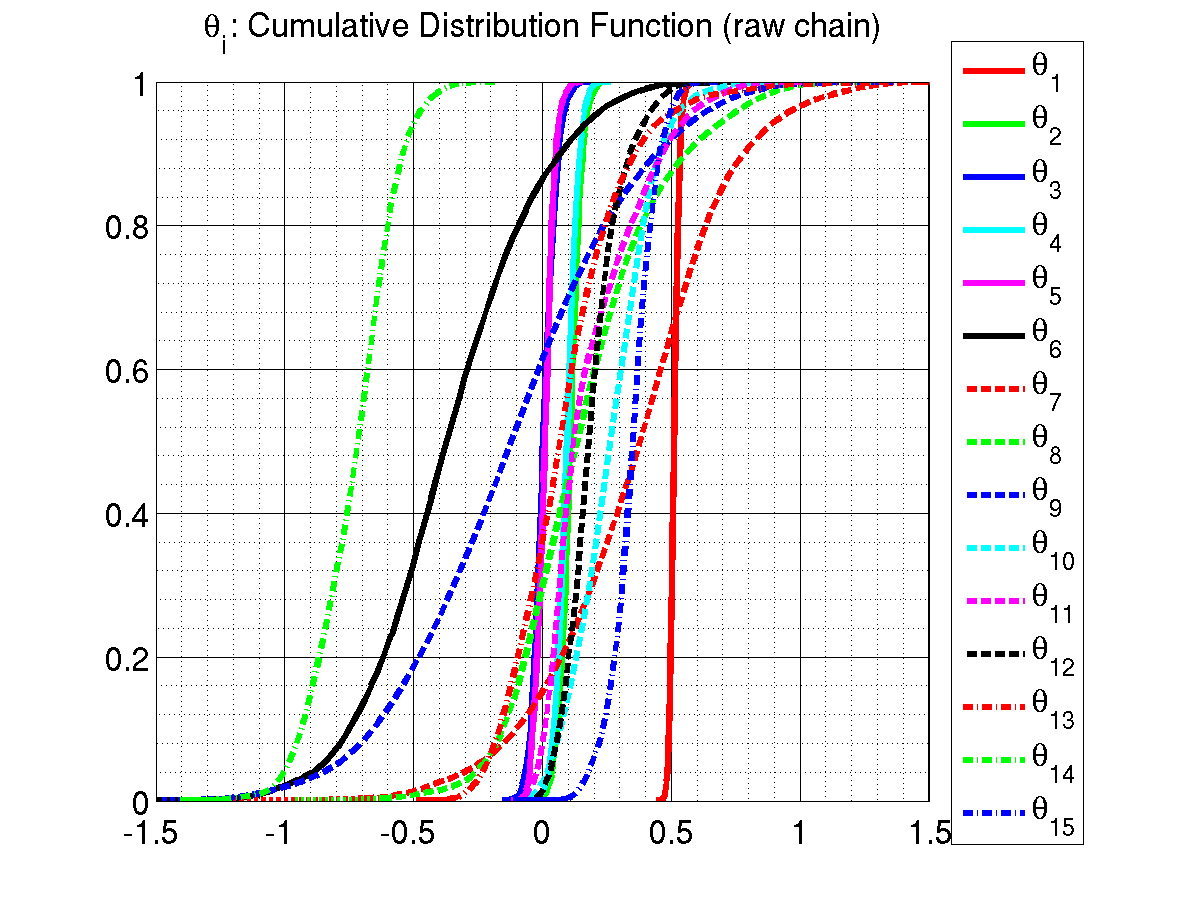
\includegraphics[scale=0.45]{figs/hysteretic_cdf_thetas.png}\label{fig:hysteretic_cdf}\hspace{-20pt}}
\subfloat[Autocorrelation]{
  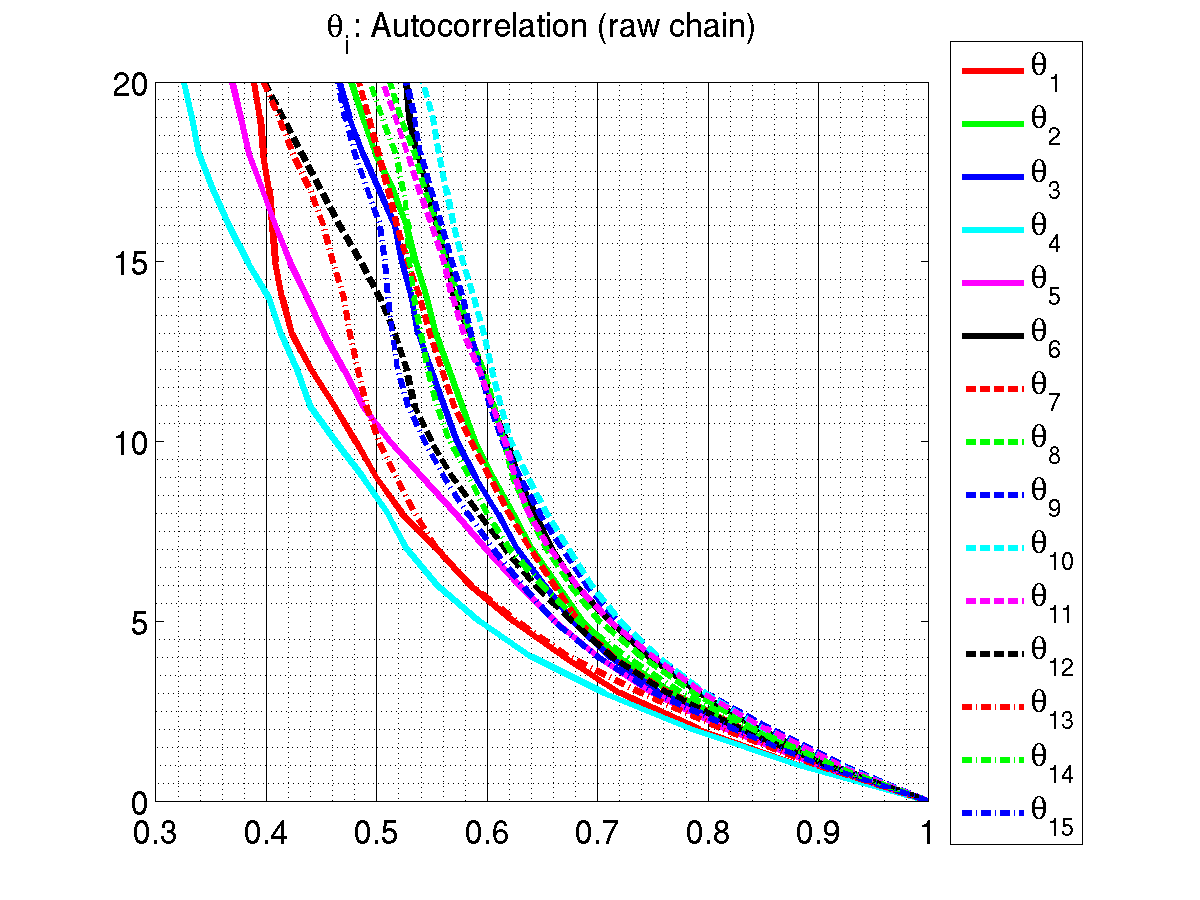
\includegraphics[scale=0.45]{figs/hysteretic_autocorr_thetas.png}\label{fig:hysteretic_autocorr}}
\vspace{-8pt}
\caption{CDF and autocorrelation plots of parameter $\bv{\theta}$ at the last level.}
\end{figure}

